\chapter{Métaux de transition et complexes}\label{ch:b2:coordination-complexes}

En 1893, un chimiste de vingt-six ans, Alfred Werner, entreprit d'expliquer une énigme.
Le chlorure de cobalt(III) forme avec l'ammoniac quatre composés, \ce{CoCl3.6NH3},
\ce{CoCl3.5NH3} et deux de formule \ce{CoCl3.4NH3}, l'un vert et l'autre violet.
Le nitrate d'argent précipite d'emblée les trois chlorures du premier, deux du
second, et un seul de chacun des deux derniers. La réponse de Werner --- six
groupes retenus autour du métal aux sommets d'un octaèdre, le reste à l'extérieur
--- fonda la chimie de coordination. Ce chapitre prolonge l'étude des complexes du
volume de première année~: leur géométrie, leurs isomères, leurs noms, et un décompte
d'électrons qui prévoit quels métaux carbonyles existent.

\begin{recall}
Le volume de première année~: complexe, atome central, ligand, ligand polydenté, chélate,
constantes de formation, coordinence~; configurations électroniques des ions des
métaux de transition (les électrons $n$s partent les premiers)~; acides et bases de Lewis,
liaisons datives~; VSEPR~; nombres d'oxydation~; énantiomères. \Cref{ch:b2:atomic-orbitals}~:
les orbitales d et l'ordre des niveaux 4s et 3d.
\end{recall}

\begin{omfigure}
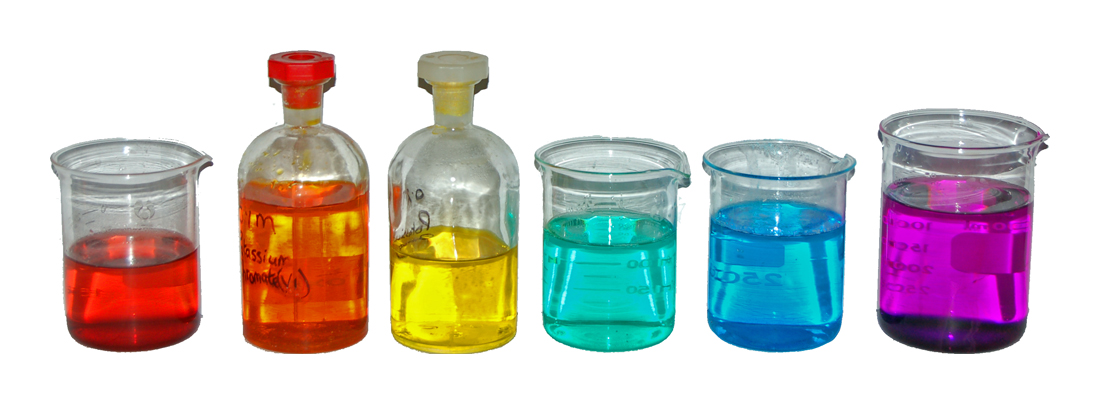
\includegraphics[width=0.8\linewidth]{images/book3/tm-solutions.jpg}

{\small Solutions aqueuses de composés de métaux de transition~: de gauche à droite,
nitrate de cobalt(II), dichromate de potassium, chromate de potassium, chlorure de nickel(II),
sulfate de cuivre(II) et permanganate de potassium. Les couleurs des solutions de cobalt, de nickel
et de cuivre proviennent de leurs aquacomplexes. (Photographie~: Benjah-bmm27,
domaine public, Wikimedia Commons.)}
\end{omfigure}

\section{Le bloc d}

\begin{definition}[Élément de transition]\label{def:b2:coordination-complexes:transition-element}
Un \emph{élément de transition}\index{element de transition@élément de transition} est un élément dont l'atome, ou
l'un des ions courants, possède une sous-couche d partiellement remplie. Un ion d'un tel élément
qui a $n$ électrons dans ses orbitales d a une \emph{configuration $d^n$}\index{configuration dn@configuration $d^n$}.
\end{definition}

\begin{proposition}[Dénombrer les électrons d]\label{prop:b2:coordination-complexes:dn}
Un ion de métal de transition $\mathrm M^{m+}$ du groupe numéro $g$ (3 à 12) a une configuration $d^n$
avec $n = g - m$.
\end{proposition}

\begin{proof}
L'atome neutre possède $g$ électrons au-delà du gaz noble qui le précède, dans les orbitales $n$s et
$(n - 1)$d. Dans les ions, les orbitales d sont au-dessous de l'orbitale s
(\cref{ex:b2:atomic-orbitals:iron})~: les $g - m$ électrons de valence restants sont tous des électrons
d.
\end{proof}

Par exemple, \ce{Fe^2+} (groupe 8) est $d^6$, \ce{Cu^2+} (groupe 11) $d^9$, \ce{Co^3+} (groupe 9)
$d^6$, \ce{Pt^2+} (groupe 10) $d^8$.

\section{Les ligands}

\begin{definition}[Denticité]\label{def:b2:coordination-complexes:denticity}
La \emph{denticité}\index{denticite@denticité} d'un ligand est le nombre de ses atomes liés au
même atome central. Un \emph{ligand monodenté}\index{ligand monodente@ligand monodenté} se lie
par un seul atome (\ce{H2O}, \ce{NH3}, \ce{Cl-}, \ce{CO}), un \emph{ligand
bidenté}\index{ligand bidente@ligand bidenté} par deux (l'éthane-1,2-diamine, notée en~; l'ion
éthanedioate, ox). Un \emph{ligand pontant}\index{ligand pontant} se lie à deux
atomes métalliques à la fois. Un \emph{ligand ambidenté}\index{ligand ambidente@ligand ambidenté} peut se lier
par l'un ou l'autre de deux atomes différents, comme l'ion nitrite (par N ou par O) ou
le thiocyanate (par S ou par N).
\end{definition}

\begin{definition}[Sphère de coordination]\label{def:b2:coordination-complexes:coordination-sphere}
La \emph{sphère de coordination}\index{sphere de coordination@sphère de coordination} d'un complexe est l'ensemble formé par
l'atome central et les ligands qui lui sont liés, écrit entre crochets~; les ions
situés hors des crochets sont des contre-ions, non liés au métal.
\end{definition}

\begin{omfigure}
\setchemfig{atom sep=2.2em}
\chemfig{M*5(-H_2N-CH_2-CH_2-NH_2-)}
\qquad
\chemfig{M*5(-O-(=O)-(=O)-O-)}
\qquad
\chemfig{N(-[:120]CH_2COO^{-})(-[:240]CH_2COO^{-})-CH_2-CH_2-N(-[:60]CH_2COO^{-})(-[:-60]CH_2COO^{-})}

\medskip
{\small Ligands chélatants. À gauche~: l'éthane-1,2-diamine (en), bidentée par ses deux
azotes. Au centre~: l'ion éthanedioate (ox), bidenté par deux oxygènes. À droite~:
l'anion edta, qui s'enroule autour d'un ion métallique avec ses deux azotes et quatre
oxygènes carboxylate (hexadenté).}
\end{omfigure}

\section{Coordinences et géométries}

Deux, quatre et six sont les coordinences les plus courantes. L'argent(I) et l'or(I) donnent
des complexes linéaires (\ce{[Ag(NH3)2]+})~; quatre ligands forment un tétraèdre
(\ce{[CoCl4]^2-}, \ce{[Zn(NH3)4]^2+}) ou un carré (\ce{[PtCl4]^2-}, \ce{[Ni(CN)4]^2-})~;
cinq, une bipyramide trigonale (\ce{Fe(CO)5})~; six, de loin le cas le plus fréquent, un
octaèdre.

\begin{omfigure}
\begin{tikzpicture}[font=\small]
  \node[omligand] at (-0.8,0) {}; \node[omligand] at (0.8,0) {};
  \draw[thick, black!70] (-0.8,0) -- (0.8,0); \node[ommetal] at (0,0) {};
  \node at (0,-1.5) {linéaire, 2};
  \pic at (3,0) {omtetrahedron}; \node at (3,-1.5) {tétraédrique, 4};
  \pic at (6,0) {omsquareplanar}; \node at (6,-1.5) {plan carré, 4};
  \pic at (9,0) {omtbp}; \node[align=center] at (9,-1.65) {bipyramide\\ trigonale, 5};
  \pic at (12,0) {omoctahedron}; \node at (12,-1.5) {octaédrique, 6};
\end{tikzpicture}

{\small Les géométries de coordination courantes (métal en orange, ligands en gris~; les liaisons
en tirets pointent derrière la page).}
\end{omfigure}

La méthode VSEPR, qui place les doublets électroniques de l'atome central aussi loin que possible les uns des autres,
échoue ici~: un ion $d^8$ comme \ce{Pt^2+} porte quatre paires d'électrons d et quatre
ligands, et pourtant ses complexes sont plans carrés, ni tétraédriques ni octaédriques. Les
électrons d ne sont pas des doublets localisés qui repousseraient les ligands~: leurs énergies dépendent
de la géométrie d'une manière que calcule le chapitre suivant.

\begin{proposition}[Les $d^8$ plans carrés]\label{prop:b2:coordination-complexes:square-planar}
Les complexes tétracoordinés des ions $d^8$ des deuxième et troisième séries de transition
(\ce{Pd^2+}, \ce{Pt^2+}, \ce{Au^3+}) sont plans carrés.
\end{proposition}

\admitted

L'explication, l'éclatement des niveaux d par les ligands, vient au
\cref{ch:b2:ligand-field}.

\section{Isomères}

\begin{definition}[Isomères des complexes]\label{def:b2:coordination-complexes:isomers}
Dans un complexe octaédrique $\mathrm{MA_3B_3}$, l'\emph{isomère fac}\index{isomere fac@isomère fac} a
les trois ligands B sur une face de l'octaèdre, l'\emph{isomère
mer}\index{isomere mer@isomère mer} sur un méridien (trois positions dans un plan passant par le
métal). Des \emph{isomères de liaison}\index{isomeres de liaison@isomères de liaison} diffèrent par l'atome par lequel
se lie un \omterm{def:b2:coordination-complexes:denticity}{ligand ambidenté}. Des \emph{isomères d'ionisation}\index{isomeres d'ionisation@isomères d'ionisation}
échangent un ligand avec un contre-ion, ce qui donne des ions différents en solution.
\end{definition}

\begin{proposition}[Dénombrer les isomères octaédriques]\label{prop:b2:coordination-complexes:isomer-count}
Dans un octaèdre, $\mathrm{MA_4B_2}$ a deux isomères (cis et trans), $\mathrm{MA_3B_3}$ deux
(fac et mer), et $\mathrm M(\mathrm{AA})_3$, à trois \omterm{def:b2:coordination-complexes:denticity}{ligands bidentés}, deux
énantiomères, $\Delta$ et $\Lambda$.
\end{proposition}

\begin{proof}
Dans un octaèdre, deux positions quelconques sont soit adjacentes (cis, $90^\circ$), soit opposées
(trans, $180^\circ$)~: deux arrangements pour les deux ligands B. Pour trois ligands B,
soit aucun couple n'est trans (ils occupent une face~: fac), soit exactement un couple est trans (le
troisième est cis par rapport aux deux autres~: mer)~; trois positions mutuellement trans n'existent pas. Pour
$\mathrm M(\mathrm{AA})_3$, chaque chélate occupe deux positions cis~; les trois chélates
s'enroulent autour de l'axe d'ordre trois comme les pales d'une hélice, tournant dans le sens des aiguilles d'une montre
ou dans le sens inverse vu selon cet axe~: deux images dans un miroir, non superposables
puisque le complexe n'a pas de plan de symétrie.
\end{proof}

\begin{omfigure}
\begin{tikzpicture}[font=\scriptsize]
  \pic (a) at (0,0) {omoctahedron};
  \node[omligand, fill=omDef!70] at (a-L1) {}; \node[omligand, fill=omDef!70] at (a-L3) {};
  \node at (0,-1.5) {\small cis-$\mathrm{MA_4B_2}$};
  \pic (b) at (3,0) {omoctahedron};
  \node[omligand, fill=omDef!70] at (b-L1) {}; \node[omligand, fill=omDef!70] at (b-L2) {};
  \node at (3,-1.5) {\small trans-$\mathrm{MA_4B_2}$};
  \pic (c) at (6.5,0) {omoctahedron};
  \node[omligand, fill=omThm!70] at (c-L1) {}; \node[omligand, fill=omThm!70] at (c-L3) {}; \node[omligand, fill=omThm!70] at (c-L5) {};
  \node at (6.5,-1.5) {\small fac-$\mathrm{MA_3B_3}$};
  \pic (d) at (9.5,0) {omoctahedron};
  \node[omligand, fill=omThm!70] at (d-L1) {}; \node[omligand, fill=omThm!70] at (d-L2) {}; \node[omligand, fill=omThm!70] at (d-L3) {};
  \node at (9.5,-1.5) {\small mer-$\mathrm{MA_3B_3}$};
\end{tikzpicture}

\medskip
\begin{tikzpicture}[font=\scriptsize]
  \foreach \xs/\s/\lab in {0/1/{$\Delta$}, 4.5/-1/{$\Lambda$}} {
    \begin{scope}[xshift=\xs cm, xscale=\s]
      \draw[black!30] (0,0) circle (1.2);
      \foreach \a in {90, 210, 330} {
        \coordinate (p) at (\a:1.1); \coordinate (q) at (\a+70:0.55);
        \draw[very thick, omDef] (\a:1.1) .. controls (\a+30:1.25) and (\a+60:0.9) .. (\a+75:0.55);
        \node[omligand] at (\a:1.1) {}; \node[omligand] at (\a+75:0.55) {};
      }
      \node[ommetal] at (0,0) {};
    \end{scope}
    \node at (\xs,-1.6) {\small \lab};
  }
  \draw[densely dashed] (2.25,-1.3) -- (2.25,1.3);
  \node[anchor=south] at (2.25,1.3) {miroir};
\end{tikzpicture}

{\small En haut~: isomères cis et trans de $\mathrm{MA_4B_2}$ (ligands B en bleu), \omterm{def:b2:coordination-complexes:isomers}{isomères fac} et mer
de $\mathrm{MA_3B_3}$ (B en rouge). En bas~: les deux énantiomères d'un tris-chélate comme
\ce{[Co(en)3]^3+}, vus selon l'axe d'ordre trois, schéma~: chaque chélate (arc
bleu) relie une position supérieure et une position inférieure, et les trois tournent dans un sens ($\Delta$) ou dans
l'autre ($\Lambda$).}
\end{omfigure}

\section{Noms et décomptes d'électrons}

\begin{method}[Nommer un complexe]\label{met:b2:coordination-complexes:naming}
\begin{enumerate}
  \item Dans la formule, écrire la \omterm{def:b2:coordination-complexes:coordination-sphere}{sphère de coordination} entre crochets, le métal
        d'abord, puis les ligands~; la charge du complexe à l'extérieur.
  \item Dans le nom, énumérer les ligands par ordre alphabétique avec des préfixes
        multiplicatifs (di-, tri-, tétra-~; bis-, tris- pour les noms de ligands complexes)~: les ligands
        anioniques se terminent en -o (chlorido, cyanido, oxydo, hydroxydo), les ligands neutres gardent
        leur nom (aqua, ammine, carbonyle).
  \item Puis le métal, avec la terminaison -ate si le complexe est un anion (ferrate,
        cuprate, cobaltate), et son nombre d'oxydation en chiffres romains.
  \item Le nom de l'anion précède celui du cation~: \ce{[Co(NH3)6]Cl3} est le
        chlorure d'hexaamminecobalt(III), \ce{K4[Fe(CN)6]} l'hexacyanidoferrate(II) de
        potassium.
\end{enumerate}
\end{method}

\begin{definition}[Décompte d'électrons]\label{def:b2:coordination-complexes:electron-count}
Le \emph{nombre d'électrons de valence}\index{nombre d'electrons de valence@nombre d'électrons de valence} d'un complexe est le
nombre d'électrons d de l'ion métallique augmenté des électrons apportés par les ligands (deux
pour chaque doublet donneur). La \emph{règle des 18 électrons}\index{regle des 18 electrons@règle des 18 électrons} énonce que
les complexes stables de métaux à bas degré d'oxydation portant des ligands $\pi$-accepteurs
fortement liants comme \ce{CO} tendent à avoir 18 électrons de valence.
\end{definition}

\begin{definition}[Hapticité]\label{def:b2:coordination-complexes:hapticity}
L'\emph{hapticité}\index{hapticite@hapticité} d'un ligand est le nombre de ses atomes liés au
métal par un même système $\pi$ continu~; on la note $\eta^n$~: un éthène lié par
sa liaison $\pi$ est $\eta^2$, un cycle cyclopentadiényle lié par ses cinq carbones $\eta^5$.
\end{definition}

\begin{method}[Décompter les électrons]\label{met:b2:coordination-complexes:electron-count}
\begin{enumerate}
  \item Attribuer des charges aux ligands comme espèces à couches complètes (\ce{Cl-}, \ce{H-},
        \ce{C5H5-}~; \ce{CO}, \ce{PR3}, \ce{NH3} neutres) et en déduire le degré d'oxydation
        du métal.
  \item Compter les électrons d du métal, $n = g - m$.
  \item Ajouter deux électrons par doublet donneur~: un doublet par \omterm{def:b2:coordination-complexes:denticity}{ligand monodenté}, six électrons pour un
        $\eta^5$-\ce{C5H5-}, six pour un $\eta^6$-benzène, deux pour un $\eta^2$-alcène.
  \item Une liaison métal--métal compte pour un électron pour chaque métal.
\end{enumerate}
\end{method}

\begin{proposition}[Les métaux carbonyles]\label{prop:b2:coordination-complexes:eighteen}
Les carbonyles binaires stables de la première série de transition, \ce{Cr(CO)6},
\ce{Fe(CO)5}, \ce{Ni(CO)4} et \ce{Mn2(CO)10}, ont tous 18 électrons de valence par atome
métallique.
\end{proposition}

\begin{proof}
Chrome(0), $d^6$, avec six CO~: $6 + 12 = 18$. Fer(0), $d^8$, cinq CO~: $8 + 10 = 18$.
Nickel(0), $d^{10}$, quatre CO~: $10 + 8 = 18$. Manganèse(0), $d^7$, cinq CO et une
liaison Mn--Mn~: $7 + 10 + 1 = 18$~; un \ce{Mn(CO)5} monomère, à 17 électrons, n'existe pas comme
composé stable, et se dimérise. La raison pour laquelle 18 est favorisé --- neuf orbitales de valence
du métal, toutes les \omterm{def:b2:diatomic-mos:bonding}{orbitales liantes} ou non liantes étant remplies --- est donnée au
\cref{ch:b2:ligand-field}.
\end{proof}

Le ferrocène, \ce{Fe(\eta^5-C5H5)2}, contient un ion fer(II) ($d^6$) entre deux
anions cyclopentadiényle, qui apportent chacun six électrons~: $6 + 12 = 18$. La règle est en défaut pour
la plupart des complexes de degrés d'oxydation élevés et pour beaucoup de complexes à ligands faibles~: \ce{[Ti(H2O)6]^3+}
a 13 électrons, \ce{[Cu(H2O)6]^2+} 21.

\begin{history}[Werner et l'octaèdre]
\begin{minipage}[t]{0.22\linewidth}
\vspace{0pt}
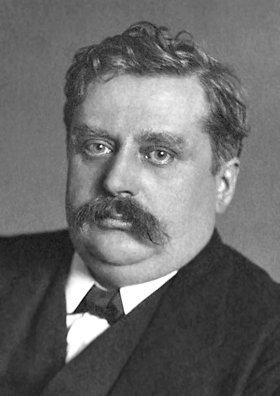
\includegraphics[width=\linewidth]{images/book3/werner.jpg}
\end{minipage}\hfill
\begin{minipage}[t]{0.74\linewidth}
\vspace{0pt}
Alfred Werner proposa en 1893 qu'un métal possède, outre sa valence, une
coordinence, nombre de groupes retenus directement autour de lui, et que le cobalt(III) en retient
six aux sommets d'un octaèdre. Il prédit ensuite combien d'isomères chaque
formule devait avoir et passa vingt ans à les préparer~; en 1911, il dédoubla un
complexe de cobalt en ses deux énantiomères, prouvant que la chiralité n'exige pas d'atome
de carbone. Il reçut le prix Nobel de chimie en 1913. (Portrait, Les Prix
Nobel, 1914, domaine public, Wikimedia Commons.)
\end{minipage}
\end{history}

\section{Exercices}

\begin{exercise}[$\star$]\label{exo:b2:coordination-complexes:1}
Donner la configuration $d^n$ de \ce{Ti^3+}, \ce{V^3+}, \ce{Cr^3+}, \ce{Mn^2+}, \ce{Fe^3+},
\ce{Co^2+}, \ce{Ni^2+} et \ce{Zn^2+}.
\end{exercise}

\begin{exercise}[$\star$]\label{exo:b2:coordination-complexes:2}
Donner la \omterm{def:b2:coordination-complexes:denticity}{denticité} de l'eau, de l'éthane-1,2-diamine, de l'ion éthanedioate, de l'edta et de
l'ion thiocyanate, et dire lequel est ambidenté.
\end{exercise}

\begin{exercise}[$\star$]\label{exo:b2:coordination-complexes:3}
Nommer \ce{[Cu(NH3)4]SO4}, \ce{K3[Fe(CN)6]}, \ce{[CoCl2(NH3)4]Cl} et
\ce{[Ni(CO)4]}.
\end{exercise}

\begin{exercise}[$\star$]\label{exo:b2:coordination-complexes:4}
Prévoir la géométrie de \ce{[Ag(NH3)2]+}, \ce{[CoCl4]^2-}, \ce{[PtCl4]^2-} et
\ce{[Fe(H2O)6]^2+}.
\end{exercise}

\begin{exercise}[$\star\star$]\label{exo:b2:coordination-complexes:5}
Combien d'isomères le complexe plan carré \ce{[PtCl2(NH3)2]} possède-t-il~? Les dessiner. (L'un d'eux,
le cisplatine, est un médicament anticancéreux.)
\end{exercise}

\begin{exercise}[$\star\star$]\label{exo:b2:coordination-complexes:6}
Compter les électrons de valence de \ce{Cr(CO)6}, \ce{Fe(CO)5}, \ce{Ni(CO)4},
\ce{V(CO)6} et \ce{Mn2(CO)10}. Lequel déroge à la règle, et comment se comporte-t-il~?
\end{exercise}

\begin{exercise}[$\star\star$]\label{exo:b2:coordination-complexes:7}
Compter les électrons de valence du ferrocène et du cobaltocène \ce{Co(C5H5)2}. Lequel est
facilement oxydé, et en quoi~?
\end{exercise}

\begin{exercise}[$\star\star$]\label{exo:b2:coordination-complexes:8}
Le complexe du nickel(II) avec l'edta a pour $\log_{10}K = 20.5$, bien plus que les complexes dans
lesquels le nickel lie six donneurs azotés ou oxygénés séparés. Expliquer cet effet chélate
par le nombre de particules libérées lorsque le chélate remplace six molécules
d'eau.
% ledger: logb:Ni-edta
\end{exercise}

\begin{exercise}[$\star\star$]\label{exo:b2:coordination-complexes:9}
Dessiner les deux \omterm{def:b2:coordination-complexes:isomers}{isomères de liaison} de \ce{[Co(NO2)(NH3)5]^2+}.
\end{exercise}

\begin{exercise}[$\star\star\star$]\label{exo:b2:coordination-complexes:10}
Combien de stéréoisomères \ce{[CoCl2(en)2]+} possède-t-il~? Lesquels sont chiraux~?
\end{exercise}

\begin{exercise}[$\star\star\star$]\label{exo:b2:coordination-complexes:11}
Pour $\mathrm{MA_4B_2}$, dénombrer les isomères prévus par un hexagone plan et par un prisme
trigonal de six ligands, et expliquer comment le nombre d'isomères trouvés permet de trancher entre les
géométries.
\end{exercise}

\begin{exercise}[$\star\star\star$]\label{exo:b2:coordination-complexes:12}
Compter les électrons de valence de \ce{[RhCl(PPh3)3]} et de \ce{[IrH(CO)(PPh3)3]}
(\ce{PPh3} donneur de deux électrons, \ce{H-} compté comme hydrure). Lequel pourrait accepter deux ligands
supplémentaires~?
\end{exercise}

\section{Problème~: les ammines de cobalt de Werner}

\begin{problem}[{Problème du week-end --- quatre ammines du chlorure de cobalt(III) et le chlorure
qu'elles libèrent, leurs formules avec crochets, les deux isomères de la tétraammine et ce
qu'ils prouvent sur la géométrie, et l'activité optique d'un tris-chélate}]
\label{pb:b2:coordination-complexes:1}
Données~: quatre composés A \ce{CoCl3.6NH3} (jaune orangé), B \ce{CoCl3.5NH3}
(pourpre), C et D \ce{CoCl3.4NH3} (vert et violet). Avec un excès de nitrate d'argent,
une mole de A précipite 3 mol de \ce{AgCl}, B 2 mol, C et D 1 mol chacun. Les conductivités
molaires indiquent 4, 3, 2 et 2 ions par entité formulaire.

\medskip
\noindent\textbf{Partie I --- Chlorures et ions.}
\begin{enumerate}
  \item Quels chlorures réagissent d'emblée avec les ions argent~?
  \item Combien de chlorures sont liés au cobalt dans chaque composé~?
  \item Confronter les nombres d'ions aux conductivités.
  \item Quel est le nombre d'oxydation du cobalt dans les quatre composés~?
  \item Quelle est sa configuration $d^n$~?
  \item Combien de ligands au total le cobalt retient-il dans chaque composé~?
\end{enumerate}

\medskip
\noindent\textbf{Partie II --- Formules et noms.}
\begin{enumerate}[resume]
  \item Écrire A, B, C et D avec des crochets.
  \item Nommer A et B.
  \item Nommer le cation de C et de D.
  \item Quel type d'isomères sont C et D~?
  \item Que serait un composé \ce{CoCl3.3NH3}, et combien d'ions donnerait-il~?
  \item Combien d'isomères ce composé aurait-il dans un octaèdre~?
\end{enumerate}

\medskip
\noindent\textbf{Partie III --- La géométrie.}
\begin{enumerate}[resume]
  \item Dessiner \ce{[CoCl2(NH3)4]+} cis et trans dans un octaèdre.
  \item Dénombrer les isomères de \ce{[CoCl2(NH3)4]+} prévus pour six ligands aux
        sommets d'un hexagone plan.
  \item Dénombrer ceux qui sont prévus pour un prisme trigonal.
  \item Werner n'en trouva jamais plus de deux. Qu'est-ce que cela prouve~?
  \item La preuve est-elle complète~? Qu'aurait signifié un troisième isomère~?
  \item Lequel de C et D est cis, sachant que l'isomère cis peut être converti en un
        chélate avec l'éthanedioate et que l'isomère trans ne le peut pas~?
\end{enumerate}

\medskip
\noindent\textbf{Partie IV --- L'activité optique.}
\begin{enumerate}[resume]
  \item Dessiner \ce{[Co(en)3]^3+}.
  \item Possède-t-il un plan de symétrie~? Un centre d'inversion~?
  \item Combien de stéréoisomères possède-t-il~?
  \item Que prouve le dédoublement d'un tel cation en énantiomères~?
  \item \ce{[CoCl2(en)2]+} est-il chiral sous sa forme cis~? Sous sa forme trans~?
  \item Pourquoi le dédoublement, par Werner, d'un complexe ne contenant aucun carbone fut-il important~?
  \item Donner le nombre d'isomères de \ce{[CoCl2(NH3)4]+} prévu par l'octaèdre,
        ainsi que par l'hexagone plan et par le prisme trigonal.
\end{enumerate}
\end{problem}
